% !TeX program = xelatex
\documentclass{article}
\usepackage{kotex}
\usepackage[a4paper, left=3cm, right=3cm, top=2.5cm, bottom=2.5cm]{geometry}
\usepackage{amsmath, amssymb}
\usepackage{tcolorbox}
\usepackage{caption}
\usepackage{setspace}
\usepackage{xcolor}
\usepackage{titlesec}
\usepackage{tikz}
\usetikzlibrary{arrows.meta}

\setstretch{1.3}
\renewcommand{\figurename}{그림}
\titleformat{name=\section,numberless}
  {\normalfont\large\bfseries\color{blue}}{}
  {0pt}{}

\title{1.4 공간에서의 반사}
\date{}
\author{}

\begin{document}
\maketitle

\section*{1.4 공간에서의 반사}

\begin{tcolorbox}[
  colback=teal!4, colframe=teal!65!black,
  title=정의 \& 핵심 규칙,
  fonttitle=\bfseries, boxrule=0.5mm, arc=3mm]

\textbf{\textcolor{teal!65!black}{정의 (공간에서의 반사).}}\quad
$\mathbb{E}^3$에서 점 $P$와 평면 $H$가 주어졌을 때, \textbf{$H$에 대한 $P$의 반사점} $P'$은
$H$에 수직이고 $P$와 등거리인 반대쪽 점이다.
\begin{itemize}\setlength\itemsep{0pt}
  \item $P$에서 $H$에 수선을 내려 발을 $M$이라 하면: $P'M = PM$, $P'$는 $H$에 대해 $P$와 반대편
  \item $P \in H$이면 $P' = P$
\end{itemize}

\noindent\textcolor{teal!50!black}{\rule{\linewidth}{0.4pt}}

\textbf{\textcolor{teal!65!black}{좌표 공식}} ($\mathbb{R}^3$에서 $xy$평면에 대한 반사):
\[
  f(x,\,y,\,z) \;=\; (x,\,y,\,-z)
\]

\end{tcolorbox}

\begin{figure}[h]
\centering
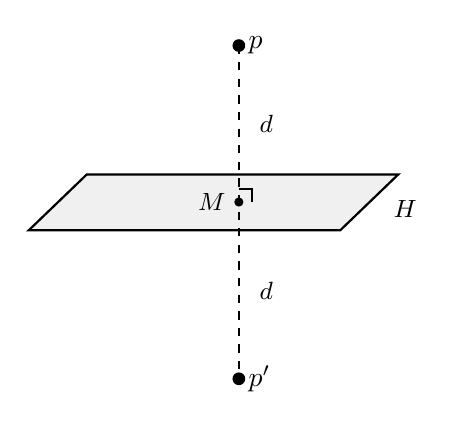
\begin{tikzpicture}[scale=0.92]
  % Plane H (parallelogram, 3D perspective)
  \draw[thick, fill=gray!12]
    (-2.5,-0.05) -- (1.8,-0.05) -- (2.6,0.72) -- (-1.7,0.72) -- cycle;
  \node[right] at (2.4,0.25) {\small $H$};

  % Perpendicular line M (vertical dashed)
  \draw[dashed, thick] (0.4,2.5) -- (0.4,-2.1);
  \node[left, font=\small] at (0.35,0.34) {$M$};

  % Foot of perpendicular on H
  \fill (0.4,0.34) circle (1.8pt);

  % P above H
  \fill (0.4,2.5) circle (2.5pt) node[right]{$p$};

  % P' below H
  \fill (0.4,-2.1) circle (2.5pt) node[right]{$p'$};

  % Right angle mark at (0.4, 0.34) — upper-right quadrant
  \draw[thick] (0.4,0.52) -- (0.58,0.52) -- (0.58,0.34);

  % d labels
  \node[right, font=\small] at (0.55, 1.42) {$d$};
  \node[right, font=\small] at (0.55,-0.88) {$d$};
\end{tikzpicture}
\caption{평면에 대한 반사}
\label{fig:1.5}
\end{figure}

\begin{tcolorbox}[
  colback=teal!4, colframe=teal!65!black,
  title=벡터 (보조 개념),
  fonttitle=\bfseries, boxrule=0.5mm, arc=3mm]

\textbf{벡터}는 $\mathbb{R}^n$에서 한 점으로부터 다른 점까지의 \textbf{유향(有向) 선분}이다.
같은 길이·방향이면 동등한 벡터로 취급한다.
\[
  \vec{v} \;=\; \overrightarrow{PQ} \;=\; Q - P, \qquad Q = P + \vec{v}, \qquad P = Q - \vec{v}
\]
$\vec{v} = (v_1, \ldots, v_n)$이라 하면 좌표로 표현하면:
\[
  T(x_1,\ldots,x_n) = (x_1+v_1,\,\ldots,\,x_n+v_n)
\]

\end{tcolorbox}

\begin{tcolorbox}[
  colback=red!4, colframe=red!60!black,
  title=정리: 반사와 향(Orientation),
  fonttitle=\bfseries, boxrule=0.5mm, arc=3mm]

\textbf{향(orientation)}이란 회전 방향의 선택이다. 반사는 항상 향을 뒤바꾼다.

\medskip
\noindent\textbf{평면($\mathbb{E}^2$)에서의 향:}
시계 방향(CW) 또는 반시계 방향(CCW) 중 하나를 선택.\\
반사 후: 시계 $\;\longleftrightarrow\;$ 반시계 (예: 반사된 글씨는 좌우 반전)

\noindent\textcolor{red!40!black}{\rule{\linewidth}{0.4pt}}

\noindent\textbf{공간($\mathbb{E}^3$)에서의 향 --- 오른손 법칙:}\\
영이 아니고 서로 평행하지 않은 세 벡터의 순서쌍 $(\vec{A},\vec{B},\vec{C})$에 대해,\\[3pt]
\hspace{1em}오른손 엄지 $\to \vec{A}$, 검지 $\to \vec{B}$, 나머지 손가락 $\to \vec{C}$ 방향이면 \textbf{양의 향},\\
\hspace{1em}나머지 손가락이 $-\vec{C}$ 방향이면 \textbf{음의 향}.\\[4pt]
반사 후: 양의 향 $\;\longleftrightarrow\;$ 음의 향

\end{tcolorbox}

\subsection*{연습문제 1.4}

\begin{enumerate}
  \item \textbf{(문제 1.4.1)}\quad
    $\mathbb{R}^3$에서 평면 $x + 2y + 3z + 4 = 0$에 대한 반사의 식을 구하여라.

  \item \textbf{(문제 1.4.2)}\quad
    모든 반사($\mathbb{E}^2$ 또는 $\mathbb{E}^3$에서)가 자기 자신의 역함수임을 보여라.\\
    즉, $f:\mathbb{E}^n \to \mathbb{E}^n$이 반사이면 ($n=2$ 또는 $3$) $f^{-1} = f$임을 보여라.
\end{enumerate}

\end{document}
